\documentclass[]{article}

\usepackage[top=2cm, bottom=2.5cm, left=2.0cm, right=2.0cm]{geometry}
\usepackage{xcolor}
\usepackage{tikz}
\usepackage{pgfplots}
\usepackage{algorithm}
\usepackage{algorithmic}
\usepackage{appendix}
\usepackage{placeins}

\newlength{\xdim}

\definecolor{calculate}{HTML}{D7191C}
\definecolor{copyBack}{HTML}{FDAE61}

%opening
\title{Multiprocessor Systems - Assignment III (OpenMP)}
\author{Adrian Holfter, Lucie Labadie}

\begin{document}

\maketitle

\section{How to run}

\paragraph{} The archive contains a \emph{Makefile}. Running \texttt{make} in the directory will create two binaries, \texttt{qsort\_par} and \texttt{gaussian\_par}.

\section{Implementation}

\subsection{OpenMP-based Quicksort}

\paragraph{} We decided to parallelize the recursive calls to \texttt{quick\_sort} by creating tasks for each call. This means that the first call to \texttt{quick\_sort} is running on only one thread. The subsequent two recursive calls are then added to the task pool and can then be executed asynchronously in parallel. Since every call to \texttt{quick\_sort} will call itself recursively two times, full utilization of e.g. eight processor cores will be reached by the fourth iteration.

\paragraph{} The \texttt{parallel} region is created in the very beginning in the \texttt{main} function and contains immediately a \texttt{single} region in order to only start \texttt{quick\_sort} once and have the other spawned threads waiting for incoming tasks. Putting the \texttt{parallel} region inside \texttt{quick\_sort} would create nested regions (through recursion), which we don't need. Similarly, putting the \texttt{single} region inside the \texttt{quick\_sort} function would force serialization of the whole process and thus limit execution to two cores.

\subsection{OpenMP-based Gaussian parallelization}

\paragraph{} Our implementation for the Gaussian elimination algorithm is based on our implementation of it for the second assignment - details on how the algorithm works can be found there.

\paragraph{} Changes made include mostly removing \textit{pthread} calls and structures and replacing them with \textit{OpenMP} declarations. During this process, we also removed the condition variable and the global mutex. Waiting is now implemented as a busy wait on a flag being set. The array containing the flags doesn't need to be guarded by a mutex, because there can only be one thread writing to each specific location of the array; all other threads are only reading the values and the value is an integral one, meaning the setting of the flag is by design atomic.

\paragraph{} In order to synchronize the array containing the flags, the \texttt{omp flush} directive was used, both after writing it and before reading it. We declared the array as \textit{shared} in the \texttt{parallel} declaration, but we observed that changes in the array were not always synchronized between threads. The cause seems to be a cache optimization from the compiler, so we hereby force the array to be synchronized across threads.

\paragraph{} The main \texttt{parallel} declaration encapsulates a \texttt{for} loop that calls \texttt{Process\_Row} for every row. We added a \texttt{schedule(static, 1)} clause in order to assign the rows in a round-robin fashion, making sure that the work load is distributed evenly. All needed global variables are declared as \texttt{shared}: The matrix, the two vectors and the array containing flags.

\section{Measurements}

The measurements were taken on the \emph{kraken.tek.bth.se} Server. The executables were compiled with the \texttt{-O2} option, to enable compiler optimizations. Measurement was done using the bash-builtin \texttt{time} command. Every measurement was taken 10 times and the smallest value was used to account for background load and operating system caches.

\subsection{OpenMP-based Quicksort}

TODO

\subsection{OpenMP-based Gaussian elimination}

TODO

Table \ref{tab:gauss-runtime} shows the runtimes of the different versions of the row-based gaussian elimination. Figure \ref{fig:gauss-chart} also visualizes this.

\begin{figure}[h]
	\centering
	\begin{tabular}{|l|r|r|}
		\hline
		\textbf{Version} & \textbf{shortest runtime [s]} & \textbf{speedup} \\
		\hline
		Sequential single-threaded		& 11.37 & 1.00 \\ 
		\hline 
		pthread 1 thread				& 8.44 & 1.34 \\ 
		\hline 
		pthread 2 threads				& 5.05 & 2.25 \\ 
		\hline 
		pthread 4 threads 				& 3.06 & 3.71 \\ 
		\hline 
		pthread 8 threads				& 2.59 & 4.39 \\ 
		\hline 
	\end{tabular} 
	\caption{Runtime comparison for gaussian elimination}
	\label{tab:gauss-runtime}
\end{figure}

\begin{figure}[h]
	\centering
	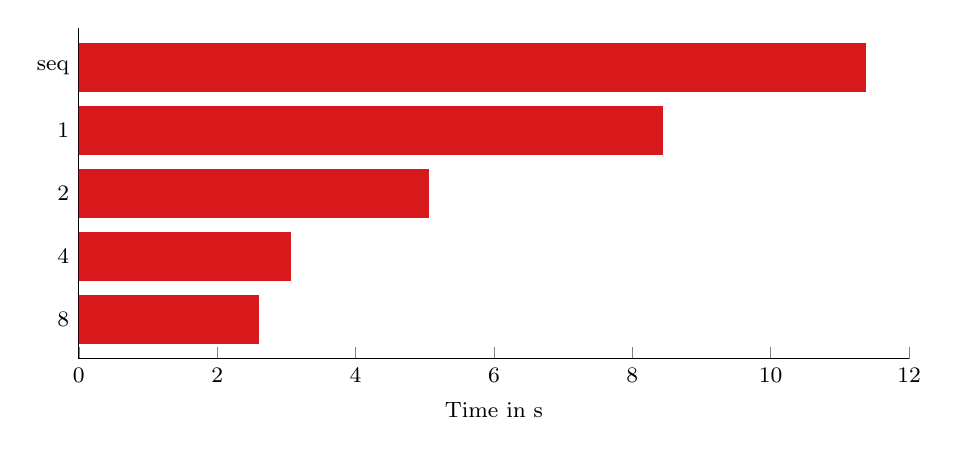
\begin{tikzpicture}
	\begin{axis}[
	xbar stacked,
	legend style={
		legend columns=4,
		at={(xticklabel cs:0.5)},
		anchor=north,
		draw=none
	},
	ytick=data,
	axis y line*=none,
	axis x line*=bottom,
	tick label style={font=\footnotesize},
	legend style={font=\footnotesize},
	label style={font=\footnotesize},
	xtick={0, 2.0, 4.0, 6.0, 8.0, 10.0, 12.0},
	width=1.0\textwidth,
	bar width=6mm,
	xlabel={Time in s},
	yticklabels={seq, 1, 2, 4, 8},
	xmin=0,
	xmax=12.0,
	area legend,
	y=8mm,
	enlarge y limits={abs=0.625},
	]
	\addplot[calculate,fill=calculate] coordinates
	{(11.37,4) (8.44,3) (5.05,2) (3.06,1) (2.59, 0)};
	\end{axis}  
	\end{tikzpicture}
	\caption{Runtime comparison chart for gaussian elimination}
	\label{fig:gauss-chart}
\end{figure}


\end{document}